% !TeX root = vpl.tex

\chap{Un robot da compagnia}\label{ch.pet}

I robot che costruiamo in questo capitolo sono chiamati \emph{robot autonomi}.
Essi mostrano un comportamento indipendente che è normalmente associato con
esseri viventi come cani e gatti. Il comportamento si ottiene tramite il
\textit{feedback} (o retroazione): il robot sente che si verifica qualcosa nel
mondo e modifica il suo comportamento di conseguenza.

\sect{Il robot ti obbedisce}

In primo luogo programmeremo il robot per obbedire. Normalmente, il robot rimarrà fermo in
un posto senza muoversi; quando rileverà la mano di fronte ad esso,
si sposterà verso la vostra mano.

Ci sono cinque sensori orizzontali di distanza sul lato anteriore del robot Thymio
e due sul retro del robot.
Sono simili a quelli sotto il Thymio che abbiamo usato nel \cref{ch.moving}.
%\footnote{Il termine tecnico è \emph{sensore di prossimità}, però si utilizzerà il semplice termine \emph{sensore di distanza orizzontale}.}
Portate la vostra mano lentamente verso i
sensori; quando si avvicina, una luce rossa apparirà attorno ai sensori
che rilevano la mano (\cref{fig.detect}).

\begin{figure}
\begin{center}
\gr{detect}{.6}
\caption{La parte anteriore del Thymio. Due sensori rilevano le dita.}\label{fig.detect}
\end{center}
\end{figure}

Il blocco \blksm{event-prox} viene utilizzato per rilevare se qualcosa è vicino al
sensore oppure no. In entrambi i casi fa in modo che un evento si verifichi. I piccoli
quadrati grigi (cinque sulla parte anteriore e due nella parte posteriore) vengono utilizzati per specificare
quando si verifica un evento. Cliccando su un quadrato esso cambia da grigio a
bianco al rosso e ritorna al grigio.
Per questo blocco, il significato di questi colori è:

\begin{itemize}[noitemsep, nosep,leftmargin=*]
\item \textbf{Grigio}: Il valore del sensore non influenza il
programma..
\item \textbf{Rosso}: Un evento si verifica quando il sensore rileva un oggetto
vicino ad esso.
\item \textbf{Bianco}: Un evento si verifica quando il sensore \emph{non} rileva un oggetto
vicino ad esso.
\end{itemize}

\importantbox[sensori del terreno e sensori orizzontali]{
Fai attenzione a non confondere il comportamento dei sensori orizzontali
con il comportamento dei sensori a terra.
\begin{itemize}[noitemsep, nosep,leftmargin=*]
\item Per i sensori orizzontali, il quadrato bianco indica che un
evento si verifica se non vi è \emph{nulla nelle vicinanze}, mentre il quadrato rosso
specifica che un evento si verifica se vi è \emph{qualcosa nelle vicinanze}.
\item Per i sensori di terra, il quadrato bianco indica che un evento
si verificherà se \emph{poca luce viene riflessa dalla superficie},
mentre il quadrato rosso indica che un evento si verifichi \emph{se molta
luce viene riflessa dalla superficie}.
\end{itemize}
Il principio fisico di questi due tipi di sensori è simile, ma a causa della loro collocazione differente il loro comportamento è diverso.
}\label {page.sensors}

Per implementare il comportamento, abbiamo bisogno di due coppie evento-azione indicate in
\cref{fig.follow-hand}. Nella prima coppia, il sensore anteriore centrale
è bianco e l'azione associata è che i motori sono spenti.
Pertanto, quando il robot non vede nulla, non si muoverà e
si fermerà se fosse stato in movimento. Nella seconda coppia, il sensore anteriore centrale è rosso e cursori del blocco motore sono trascinati verso l'alto.
Pertanto, quando portate la mano vicino alla parte anteriore del robot, si verifica un evento che induce entrambi i motori a funzionare piuttosto velocemente e il robot a muoversi in avanti.

\begin{figure}
\begin{floatrow}
	\ffigbox
	{\caption{Muoversi verso la vostra mano}\label{fig.follow-hand}}
	{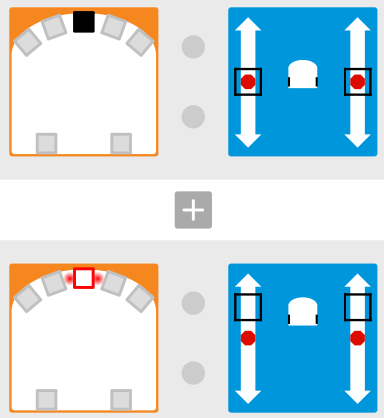
\includegraphics[width=.4\textwidth]{likes-forward}}
	\ffigbox
	{\caption{Un bulldozer con cingoli}\label{fig.bull}}
	{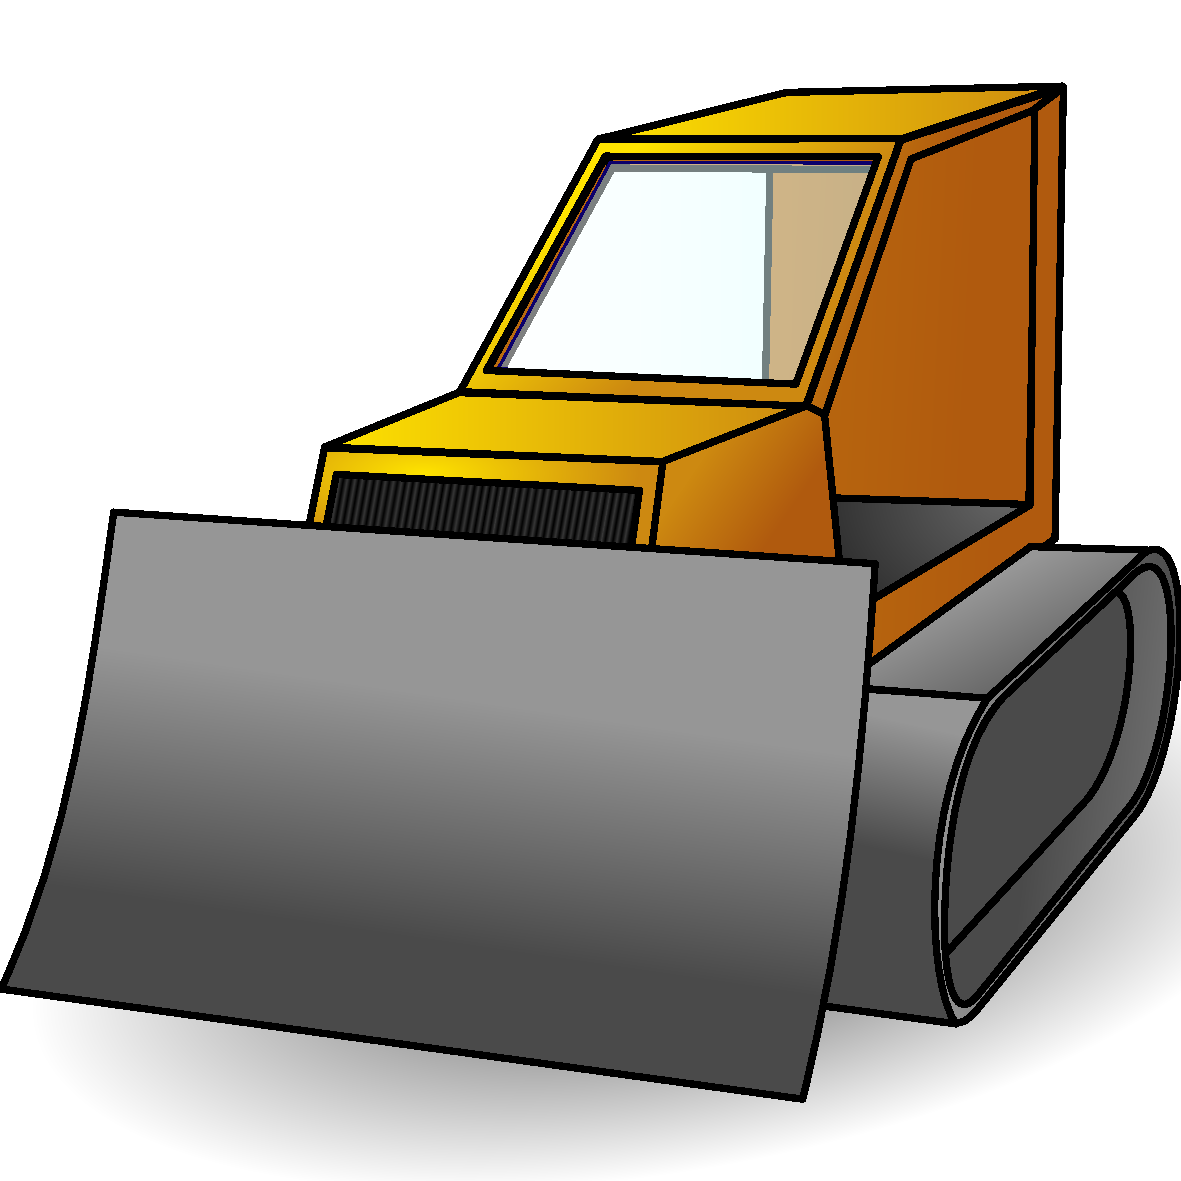
\includegraphics[width=.35\textwidth]{bulldozer}}
\end{floatrow}
\end{figure}


\sect{Guidare il robot Thymio}

Il robot Thymio non dispone di un volante come una macchina o di un
manubrio come una bicicletta. Così come può girare? Il robot usa una
\emph{guida differenziale}, che è comunemente utilizzata da veicoli cingolati come il
bulldozer (\cref{fig.bull}). Invece di girare un manubrio in una
direzione desiderata, i cingoli o le ruote di sinistra e destra sono guidati da
motori individuali a \emph{diverse} velocità. Se il cingolo di destra si muove
più velocemente di quello di sinistra, il veicolo gira a sinistra, e se il cingolo di sinistra
si muove più velocemente di quello di destra, il veicolo gira a destra.

In VPL è possibile implementare la guida differenziale sul robot Thymio
impostando i cursori sinistro e destro di un blocco di azione Motori, e quindi le velocità delle ruote, a
diversi valori.
Maggiore è la differenza tra le due velocità, più stretta è la curva. Per
realizzare una grande differenza di velocità, si può far girare una ruota in avanti
e una indietro. In questo caso, se una ruota avanza ad una
certa velocità, mentre l'altra gira all'indietro alla \emph{stessa}
velocità, il robot Thymio gira sul posto.
Ad esempio, nel blocco di azione motori \blksm{differential}, il cursore sinistro ha
fissato una velocità veloce indietro, mentre il cursore a destra ha fissato
una velocità in avanti veloce.
Il risultato è che il robot girerà a sinistra, come indicato dalla piccola immagine del robot.

Esperimento con una coppia evento-azione come ad esempio: \blkc{turning}

Imposta i cursori sinistro e destro, esegui il programma
e toccare il pulsante centrale; per fermare il robot click su \blksm{stop}.
Ora è possibile cambiare i cursori e riprovare.

\trickbox{
L'icona di Thymio del blocco azione motori mostra al centro un'animazione del movimento del robot quando si spostano i cursori.}


\sect{Al robot piacete}

Un vero e proprio animale domestico ti segue in giro. Per fare in modo che il robot segua la mano, aggiungere
due ulteriori coppie evento-azione: se il robot rileva un oggetto davanti al suo sensore più a sinistra, si gira a sinistra, mentre se rileva
un oggetto di fronte al suo sensore più a destra, si gira a destra.


{\raggedleft \hfill File di programma \bu{likes.aesl}}

Il programma per il robot che ti segue è costituito da due coppie di eventi-azione, come mostrato in \cref{fig.likes}.
Esperimentare con i cursori su ogni blocco di azione motori.

\begin{figure}
	\subfigure[Al robot piacete]{
		\label{fig.likes}
		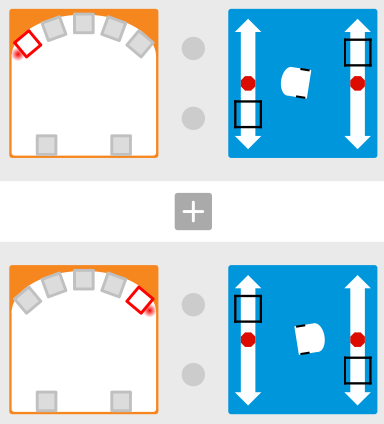
\includegraphics[width=.4\textwidth]{likes-turns}
	}
	\hfill
	\subfigure[Al robot non piacete]{
		\label{fig.hates}
		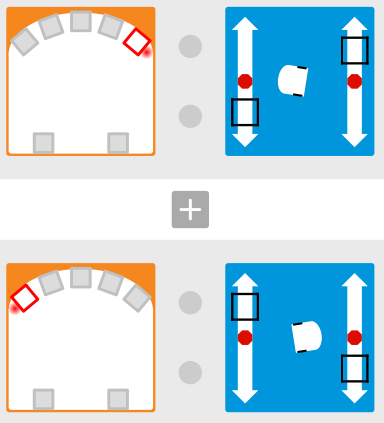
\includegraphics[width=.4\textwidth]{hates}
	}
	\caption{Programmi per il robot da compagnia}
\end{figure}

\exercisebox{\thechapter.1}{
Modificare il comportamento del robot da compagnia in modo che inizi a muoversi in avanti quando il programma
viene eseguito e si fermi quando rileva il bordo di un tavolo (o una striscia di nastro adesivo nero).}

Come spiegato in \cref{ch.moving}, molta luce sarà riflessa
da una superficie bianca, mentre pochissima luce viene riflessa da una
superficie nera.
Dovrete sperimentare con il blocco sensore orizzontale per determinare quando cliccare su un quadrato bianco e quando su un quadrato rosso, a seconda del piano del tavolo o dove si posiziona il robot.


\exercisebox{\thechapter.2}{
Che cosa succede se si cambia l'ordine delle
coppie evento-azione che avete usato nell'esercizio precedente?
}


\sect{Al robot non piacete}

A volte il vostro animale domestico può essere di cattivo umore e si allontana dalla tua mano.
Scrivere un programma che riproduce questo comportamento nel robot.

{\raggedleft \hfill File di programma \bu{does-not-like.aesl}}

Aprire il programma per l'animale domestico che ti ama e scambiare l'associazione
degli eventi con le azioni. Il rilevamento di un ostacolo dal sensore di sinistra
farà in modo che il robot giri a destra, mentre il rilevamento di un ostacolo dal sensore di destra farà sì che il robot svolti a sinistra, come mostrato in \cref{fig.hates}.

% \begin{figure}[htb]
% \begin{center}
% \gr{hates}{0.4}
% \caption{Al robot non piacete}\label{fig.hates}
% \end{center}
% \end{figure}

\exercisebox{\thechapter.3}
{
Esperimento con i sensori.
I sensori anteriori orizzontali sono numerati 0, 1, 2, 3, 4 dalla sinistra del robot alla sua destra.
Il sensori posteriori sono numerate 5 per il sinistro e 6 per quella di destra.
Invece di utilizzare sensori 0 e 4 come prima:
\begin{itemize}[noitemsep,nosep,leftmargin=*]
\item Usare sensori 1 e 3 per girare il robot a destra e a sinistra,
rispettivamente.
\item Usare entrambi i sensori 0 e 1 per girare il robot a sinistra e entrambi i sensori 3
e 4 per girare il robot a destra.
\item Aggiungi coppie evento-azione per i sensori posteriori 5 e 6.
\end{itemize}
}

\sect{Impostare i cursori con precisione (avanzato)}

È difficile impostate i cursori con precisione in modo che, per esempio, entrambi i
motori funzionino alla stessa velocità. Osservando la traduzione delle
coppie evento-azione in un programma di testo è possibile migliorare la precisione.
La \Cref{fig.textcode} mostra il programma in cui il robot ti segue in giro insieme con la traduzione del testo a destra della finestra VPL.
Questo testo viene modificato automaticamente quando si modificano le coppie evento-azione.

\begin{figure}
\includegraphics[width=0.3\textwidth]{follow4}
\hfill
\begin{minipage}[b]{0.6\textwidth}
\footnotesize
\begin{lstlisting}
onevent prox # ogni 10 secondi
	if prox.horizontal[2] < 400 then
		motor.left.target = 0
		motor.right.target = 0
	end
	if prox.horizontal[2] > 500 then
		motor.left.target = 300
		motor.right.target = 300
	end
	if prox.horizontal[0] > 500 then
		motor.left.target = -300
		motor.right.target = 300
	end
	if prox.horizontal[4] > 500 then
		motor.left.target = 300
		motor.right.target = -300
	end
\end{lstlisting}
\end{minipage}
\caption{Un programma VPL e il corrispondente programma testuale.}
\label{fig.textcode}
\end{figure}

La linea \p{onevent prox} significa: ogni volta che l'evento di campionamento dei sensori di prossimità orizzontale (abbreviato \emph{prox}) ha luogo (avviene 10 volte al secondo), le linee che seguono verranno eseguite.

Quando l'evento avviene, Thymio controlla i valori dei sensori utilizzando una condizione del tipo \p{if} \ldots \ \p{then} \ldots \ \p{end}.
Si inizia testando il sensore 2 (centrale anteriore), come si vede da \p{prox.horizontal[2]}.
Se questo valore è inferiore a 400, allora Thymio imposta le velocità del motore destro e sinistro a 0 con i comandi 
\p{motor.left.target = 0} e \p{motor.right.target = 0}.
Ogni blocco \p{if} \ldots \ \p{then} \ldots \ \p{end} verifica un sensore specifico ed esegue o meno l'azione associata, in funzione del risultato del test.
Quindi corrisponde ad una coppia evento-azione:
\begin{enumerate}[start=0,noitemsep,nosep]
\item test se non c'è qualcosa di fronte; se questo è vero, Thymio si ferma.
\item test se qualcosa è di fronte; se questo è vero, Thymio va avanti.
\item test se c'è qualcosa a sinistra; se questo è vero, Thymio gira a sinistra.
\item test se c'è qualcosa a destra; se questo è vero, Thymio gira a destra.
\end{enumerate}
Infine, una volta che il Thymio ha letto tutti questi sensori, attende il prossimo evento \p{prox}  e ricomincia questi test, indefinitamente.

Per scrivere programmi in modalità testo, usare l'ambiente AsebaStudio (\cref{ch.next}).

\trickbox{Spostando i cursori sui blocchi azione motori, vedrete che le velocità dei motori (\p{motor.X.target}) cambia a passi di 50 nella gamma da $-$500 a 500.
Spostando con attenzione i cursori, è possibile impostare le velocità per uno qualsiasi di questi valori.
}
